\def \unitsquare {rectangle+(0.4,0.4)}
\def \unitrow [#1][#2][#3][#4]{\foreach \x in {#1, #2, ..., #3} \draw (\x,#4)\unitsquare;}
  %Syntax for \unitrow[starting x coordinate for row][interval setter][end x coordinate][y coordinate for row]%
  %incongruities between the syntax and the output appear due to compiler error - some funny looking numbers below correspond to proper looking results on my system and may need adjusting back to what they should be if the compile on a more updated system does not run into these errors%
\begin{tikzpicture}
\draw(0,0)\unitsquare;
\end{tikzpicture}
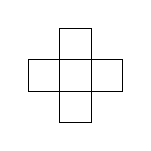
\begin{tikzpicture}
\draw(0,.4)\unitsquare;
\unitrow[-.4][0][.4][0]
\draw(0,-.4)\unitsquare;
\end{tikzpicture}
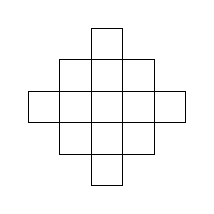
\begin{tikzpicture}
\draw(0,.8)\unitsquare;
\unitrow[-.4][0][.4][.4]
\unitrow[-.8][-.4][1.2][0]
\unitrow[-.4][0][.4][-.4]
\draw(0,-.8)\unitsquare;
\end{tikzpicture}
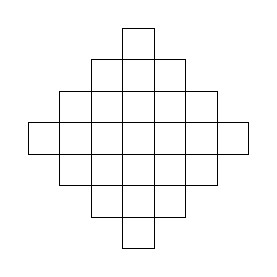
\begin{tikzpicture}
\draw(0,1.2)\unitsquare;
\unitrow[-.4][0][.4][.8]
\unitrow[-.8][-.4][1.2][.4]
\unitrow[-1.2][-.8][1.2][0]
\unitrow[-.8][-.4][1.2][-.4]
\unitrow[-.4][0][.4][-.8]
\draw(0,-1.2)\unitsquare;
\end{tikzpicture}
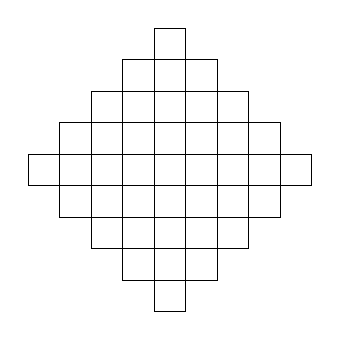
\begin{tikzpicture}
\draw(0,1.6)\unitsquare;
\unitrow[-.4][0][.4][1.2]
\unitrow[-.8][-.4][1.2][.8]
\unitrow[-1.2][-.8][1.2][.4]
\unitrow[-1.6][-1.2][2][0]
\unitrow[-1.2][-.8][1.2][-.4]
\unitrow[-.8][-.4][1.2][-.8]
\unitrow[-.4][0][.4][-1.2]
\draw(0,-1.6)\unitsquare;
\end{tikzpicture}

The first five pictures in a series of compositions made with unit squares are shown above.  If the series were to continue to the $20^{th}$ picture, how many unit squares would be in that $20^{th}$ picture?


\ifsat
	\begin{enumerate}[label=\Alph*)]
		\item $400$
		\item $761$%
		\item $2,870$
		\item $1,048,573$
	\end{enumerate}
\else
\fi

\ifacteven
	\begin{enumerate}[label=\textbf{\Alph*.},itemsep=\fill,align=left]
		\setcounter{enumii}{5}
		\item $400$
		\item $761$%
		\item $841$
		\addtocounter{enumii}{1}
		\item $2,870$
		\item $1,048,573$
	\end{enumerate}
\else
\fi

\ifactodd
	\begin{enumerate}[label=\textbf{\Alph*.},itemsep=\fill,align=left]
		\item $400$
		\item $761$%
		\item $841$
		\item $2,870$
		\item $1,048,573$
	\end{enumerate}
\else
\fi

\ifgridin
 $761$%
		
\else
\fi

